\documentclass{article}
\usepackage[paperwidth=8.5cm, paperheight=5cm, margin=0in]{geometry}
\usepackage{tikz}
\usetikzlibrary{calc,patterns,decorations.pathmorphing,decorations.markings}
\usetikzlibrary{arrows}


\newcommand{\masswidth}{.8cm}
\newcommand{\massheight}{0.6cm}
\newcommand{\wallthickness}{0.25cm}
\newcommand{\figwidth}{4.1cm}
\newcommand{\springlength}{\figwidth-2*\wallthickness-3*\masswidth}
\newcommand{\halfspringlength}{\figwidth/2-\wallthickness-3*\masswidth/2}
%\newcommand{\springlength}{1.5cm}
\newcommand{\leftwalleastpos}{0}
%\newcommand{\leftwalleastpos}{-{3cm}}
\newcommand{\massonepos}{\springlength+\masswidth/2}
\newcommand{\masstwopos}{\massonepos+\masswidth+\springlength}
\newcommand{\massthreepos}{\masstwopos+\springlength+\masswidth}
\newcommand{\rightwallpos}{\massthreepos+\springlength+\masswidth/2}
\newcommand{\konepos}{\halfspringlength}
\newcommand{\konetwopos}{\massonepos+\halfspringlength+\masswidth/2}
\newcommand{\ktwothreepos}{\masstwopos+\masswidth/2+\halfspringlength}
\newcommand{\kthreepos}{\massthreepos+\halfspringlength+\masswidth/2}
\newcommand{\midlowlevel}{-.8cm}
\newcommand{\lowerlevel}{-1.6cm}
\newcommand{\ktwopos}{\springlength+2*\masswidth/3}
\newcommand{\konethreex}{\massonepos+\springlength+2*\masswidth}
\newcommand{\wally}{-.8cm}

\begin{document}



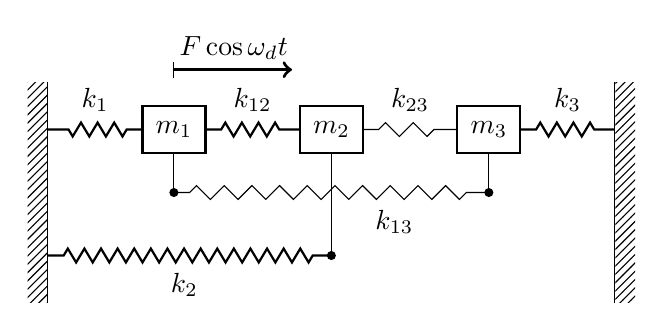
\begin{tikzpicture}[]
\tikzstyle{spring}=[thick,decorate,decoration={zigzag,pre length=0.2cm,post length=0.2cm,segment length=6}]
\tikzstyle{weakspring}=[decorate,decoration={zigzag,pre length=0.2cm,post length=0.2cm,segment length=10}]
\tikzstyle{wall}=[fill,pattern=north east lines,draw=none,minimum width=\wallthickness,minimum height=2.8cm]


\node (leftwall)  [wall, xshift=\leftwalleastpos, yshift=\wally,anchor=east] {};
\draw (leftwall.north east) -- (leftwall.south east);

\node(M1)  [minimum width=\masswidth,minimum height=\massheight, xshift=\massonepos, style={draw,outer sep=0pt,thick}] {$m_1$};

\node(M2)  [minimum width=\masswidth,minimum height=\massheight, xshift =\masstwopos,style={draw,outer sep=0pt,thick}] {$m_2$};

\node(M3)  [minimum width=\masswidth,minimum height=\massheight, xshift =\massthreepos,style={draw,outer sep=0pt,thick}] {$m_3$};

\node(rightwall)[wall, xshift =\rightwallpos,yshift=\wally,anchor=west]{};
\draw (rightwall.north west) -- (rightwall.south west);

\draw [spring] (M1.west)  -- (\leftwalleastpos,0);
\node [above] at (\konepos,.1cm) {$k_1$};
\draw[spring](M1.east)--(M2.west);
\node [above] at (\konetwopos,.1cm) {$k_{12}$};
\draw[weakspring](M2.east)--(M3.west);
\node [above] at (\ktwothreepos,.1cm) {$k_{23}$};
\draw[spring](M3.east)--(\rightwallpos,0);
\node [above] at (\kthreepos,.1cm) {$k_{3}$};

\draw [fill] circle [radius=.05cm, xshift=\masstwopos, yshift=\lowerlevel] {};  % xshift to match m2
\draw (M2.south)--(\masstwopos,\lowerlevel);
\draw[spring] (\leftwalleastpos, \lowerlevel) -- (\masstwopos, \lowerlevel);
\node[below] at (\ktwopos,\lowerlevel-.1cm) {$k_2$};

\draw [fill] circle [radius=.05cm, xshift=\massonepos, yshift=\midlowlevel] {};  % xshift to match m1
\draw(M1.south)--(\massonepos,\midlowlevel);
\draw [fill] circle [radius=.05cm, xshift=\massthreepos, yshift=\midlowlevel] {};  % xshift to match m3
\draw(M3.south)--(\massthreepos,\midlowlevel);
\draw[weakspring] (\massonepos,\midlowlevel) -- (\massthreepos,\midlowlevel);
\node[below] at (\konethreex,\midlowlevel-.1cm) {$k_{13}$};


\newcommand{\arrowheight}{.76cm}
\node[ anchor=west] at (\massonepos - .05 cm, 1.03 cm) {$F \cos \omega_d t$};
\draw[very thick,->](\massonepos,\arrowheight) --(1.5cm+\massonepos,\arrowheight);
%\draw (M1.north)--(\massonepos, 1 cm); % option 1
\draw (\massonepos, \arrowheight - .1cm)--(\massonepos, \arrowheight+.1cm); % option 2


%\draw [spring] (leftwall.east) -- (leftwall.east+1cm){k1};

\end{tikzpicture}


\end{document}